% Drawing 148/02-15 -- folder 148, batch 02, archive page 33 (PDF page 34).
% Transcription: à droite, une sphère : deux pôles marqués et trois points sur l'équateur, un à l'avant et deux à l'arrière (en tirets).
% Kind: sphere with two poles and three points on the equator. Method 2 (schematic redraw from the facsimile). Status: ok.
% Notes: Ink. The outline, a dot at the top and one at the bottom (the poles, placed just inside the outline as on the page), the equator with its front arc solid and its back arc dashed, one dot on the front and two on the back. Redrawn 2026-11-12 (issue 128): to check again.
% Coordinates: 1 unit = 1 mm = 1/100 of the crop width, y downwards as on the crop (bbox in page fractions: [0.72, 0.785, 0.86, 0.86]).
% Redrawn by Claude (claude-fable-5-2), issue #128, 2026-11-12; not checked by a human; not compiled (no TeX in the session).
% Rights: reproduces part of the work -- behind RENDER_TRANSCRIPTS, never published by itself.
\documentclass[tikz,border=3pt]{standalone}
\usepackage{amsmath,amssymb}
\usetikzlibrary{patterns,arrows.meta}
\tikzset{pencil/.style={black!45}, struck/.style={black!35}, mpt/.style={circle,draw,inner sep=1.3pt}, pt/.style={circle,fill,inner sep=0.9pt}, opt/.style={circle,draw,fill=white,inner sep=1.1pt}, Rd/.style={red!75!black}, Gn/.style={green!45!black}, Br/.style={brown!70!black}}
\begin{document}
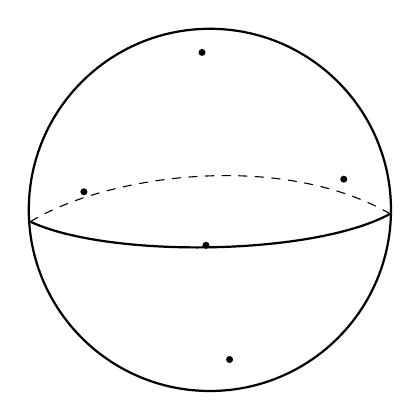
\begin{tikzpicture}[x=1mm,y=-1mm,line cap=round,line join=round,font=\small]
\draw[thick] (31,42.5) circle [radius=23];
\node[pt] at (30,22.5) {};
\node[pt] at (33.5,61.5) {};
\draw[thick] (8.2,44) .. controls (18,48.6) and (44,48.4) .. (53.9,43);
\draw[dashed] (8.2,44) .. controls (18,38) and (40,35) .. (53.9,43);
\node[pt] at (30.5,47) {};
\node[pt] at (15,40.2) {};
\node[pt] at (48,38.6) {};
\end{tikzpicture}
\end{document}
